%%%%%%%%%%%%%%%%%%%%%%%%%%%%%%%%%%%%%%
% HAPRE-CROWN DCC 2027 submission (draft -> camera-ready)
%%%%%%%%%%%%%%%%%%%%%%%%%%%%%%%%%%%%%%
\documentclass[smallabstract,smallcaptions]{dccpaper}

\usepackage{amsmath}
\usepackage{amssymb}
\usepackage{color}
\usepackage{url}
\usepackage{booktabs}
\usepackage{graphicx}

\newlength{\figurewidth}
\newlength{\smallfigurewidth}
\setlength{\smallfigurewidth}{2.75in}
\setlength{\figurewidth}{6in}


\begin{document}

\title
{\large
\textbf{From Pixels to Proof:\\ A Lossless Image-Compression Campaign from HAPRE-C to CROWN6}
}

\author{%
Author TBD\\[0.25em]
{\small Affiliation TBD} \\ {\small \url{email@address}}
}

\maketitle
\thispagestyle{empty}

\begin{abstract}
We report a 35-cycle lossless image-compression campaign from a tiny
streaming codec to CROWN6, an exact integer codec at 3.1978 bits per
subpixel on seven Kodak images, with byte-asserted round-trips. Seven
widely-used baselines fall to paired Wilcoxon tests; FLIF, JPEG-XL at two
efforts, and tuned learned codecs stand, with losses disclosed at the same
rigor as wins. A stacked classical ceiling with leave-one-out marginals
marks where hand contexts end, and a mechanism-backed negative atlas maps
where not to drill. All streams, code, and ledgers are banked
(\verb|CHECKSUMS.txt|, \verb|docs/VERIFY_report.md|, \verb|src/*_FORMAT.md|;
git history in-repo; public URL deferred to camera-ready).
\end{abstract}

\Section{Introduction}

Lossless image compression has two attractors. Heavyweights win ratio with
learned contexts and adaptive entropy coding, while lightweights win speed and
portability. The lightweight exact-codec segment has barely moved since
WebP-lossless: edge CPUs still ship PNG because nothing tiny beats it safely.

This paper is a campaign report. Our question was narrow: how far can an
integer-only, table-explicit codec with streaming decode go on real photos (Kodak) if
every byte is counted and every round-trip is asserted? Throughout, a
\emph{boss} is a widely-used baseline configuration, \emph{KO} means average
win plus majority wins plus two-sided Wilcoxon $p<.05$ ($n=7$), and
\emph{standing} means the boss held under that rule. Ties are excluded from
the majority denominator and zero-difference pairs are dropped from the
Wilcoxon (exact $p$; $n=7$ floor $p=.016$).

The answer has three parts. First, a codec lineage that earns its bytes:
from HAPRE-C up to CROWN6-exact (via CROWN-huff, CROWN-rans-hc,
CROWN2 and CROWN4), each step gated by exact assembled bytes.
Second, an empirical ceiling: stacking every proven
classical mechanism reaches 3.2515 avg, and leave-one-out shows only
backend-choice and LOCO-partition carry large marginals. Third, a full
negative-results section: failed families retire with measured mechanisms,
so the next worker need not replicate our search.

Disclosure rules govern the whole paper: (i) losses with the same rigor as
wins; (ii) every number labeled exact-codec (E) vs probe-level (P);
(iii) no beaten-boss claim beyond its Wilcoxon statistic; (iv) all
load-bearing digits recomputed from banked ledgers pre-submission.

\Section{Related Work}

\SubSection{Classical lineage: the tools we used}

\emph{PNG / DEFLATE} (4.75 bpp here, E): LZ77 + Huffman on bytes, no
cross-channel decorrelation. \emph{JPEG-LS / LOCO-I}~\cite{weinberger2000loco}:
MED + Golomb + run mode + per-context bias + 365 merged gradient contexts;
full LOCO-I under Golomb gains $-9.9\%$ over MED+Golomb (P), while under
Huffman the bias adapter is empirically null (probe b8, $\sim$0 over 7 images and 0/126 cells). Measured JPEG-LS (CharLS 2.4.4, RGB) scores 4.5757 (E) on our seven;
a YCoCg-R ablation at 3.3664 isolates our front end's contribution.
\emph{CALIC}~\cite{wu1997calic}: GAP + compound contexts; GAP16 survives
into our expert bank. \emph{WebP-lossless}: LZ77 + color cache + Huffman;
m0/m3/m6 are Bosses 1--3. \emph{FLIF / MANIAC}~\cite{sneyers2016flif}:
signaled trees, per-leaf histograms, sharing; FLIF v0.4 measured 2.9699 (E)
on our seven, beating us 0W-7L --- a standing boss stronger than JXL-e3 here.
\emph{JPEG 2000}~\cite{skodras2001jpeg}: the transform-bitplane ideal; our
stripped bitplanes without EBCOT's trio lose by $+26\%$ (P).

\SubSection{Learned lossless: the ceiling we do not claim}

Normalized to bpsp --- papers quoting total bpp divided by 3:

\begin{table}[h]
\centering\small
\caption{Learned SOTA on full-24 Kodak (literature; train data and compute matter --- see notes).}
\label{tab:learned}
\begin{tabular}{@{}lcp{2.7in}@{}}
\toprule
Model & Kodak (bpsp) & Note \\
\midrule
CALLIC~\cite{li2024callic} & 2.54 & LoRA MDL adapt; 575K; enc 9.7\,s \\
HPAC-FT~\cite{li2025hpac} & 2.52 & SARP-FT T=50; 677K; enc 0.9\,s \\
SEEC~\cite{zheng2026seec} & 2.84 & DLPR backbone + masks \\
P$^2$-LLM~\cite{chen2024pllm} & 2.83 & 8$\times$A800; dec $\sim$273\,s \\
DLPR~\cite{bai2024dlpr} & 2.86 & 22.2M; dec 1.8\,s GPU \\
Ours (CROWN6-exact) & 3.1978 (E) & C dec 0.1--0.35\,s CPU \\
\bottomrule
\end{tabular}
\end{table}

Classical full-24 anchors for orientation: JPEG-LS 2.82, CALIC 2.87, FLIF
2.72, JPEG-XL 2.63--2.88 (version spread; ours e9 3.03 sits inside on our
subset with cjxl 0.11.2). We do not claim the neural SOTA. We claim the
strongest fully-counted classical-plus-micro-neural exact codec in this
campaign: 60.7\% of the way from JXL-e1 (3.72) to DLPR (2.86) (43.5\% to the
best listed endpoint, HPAC-FT 2.52).

\SubSection{JPEG-XL as bosses~\cite{alakuijala2019jxl}}

Reproduced with \texttt{cjxl -d 0 -e E} (exact bytes):

\begin{table}[h]
\centering\footnotesize
\caption{JXL effort ladder, Kodak-7 avg (row = AVG; E). e7 beats e9 on 3/7 (overfit).}
\label{tab:jxl}
{\setlength{\tabcolsep}{4pt}\begin{tabular}{@{}ccccccccc@{}}
\toprule
e1 & e2 & e3 & e4 & e5 & e6 & e7 & e8 & e9 \\
\midrule
3.72 & 3.54 & 3.23 & 3.21 & 3.19 & 3.09 & 3.04 & 3.04 & 3.03 \\
\bottomrule
\end{tabular}}
\end{table}

Mechanism map: e1$\to$e2 $-4.8\%$ (RCT-6 on + ANS); e2$\to$e3 $-8.8\%$
(Gradient-to-Weighted switch + fixed tree); e4 MA-tree learning on; e5 per-group
RCT; e5$\to$e6 $-3.1\%$ (more RCT + wider MA); e7$\to$e8 $+0.06\%$
regression (overfit); e8$\to$e9 $-0.4\%$ (4.4$\times$ time). Weaknesses with
local evidence: 1024-groups beat 256-groups everywhere (e9 3.03$\to$2.99);
fixed-RCT search beaten by one fixed RCT (e3-C27 3.2083); tuned-e9 ceiling
$\approx$2.94. The full ladder, knock-outs, and repro commands are in the takedown ledger.

\Section{Method: HAPRE-C to CROWN6}

\SubSection{Front end}
\textbf{YCoCg-R (integer, reversible)} with floor division for negatives;
inverse asserted per image; residual alphabet bounded $|r|\le702$ (observed
range; decoder asserts the wider $|r|\le1024$) loudly, decoder never clips. \textbf{Global RCT bank} over
\{C6, C27, C12\} (2 flag bits): $-1.41\%$ MED-frame (P, 7/7 p=.016); per-block
RCT dead (fragmentation). \textbf{Borders:} dual doctrine audited (b4-style
for E16/keys/GRID; zero-TL for WAVG/LMS/MLP); encoder $==$ decoder exactly.

\SubSection{Prediction: MED to E20}
LOCO-365 contexts (gradients quantized at 3/7/21, sign-flipped residuals);
auto-K/WIDE-K quantile clustering (equal-pixel greedy + hillclimb refine) vs
GRID M-THR dictionary, per-channel exact-byte competition. Expert bank:
E16 (MED, directional, GAP, gradient forms) + WAVG-17th (per-G32 LS-4tap,
$\times$16 quantized, MDL gate $N\log_2(b_{med}/b_w)>21$) + LMS5 pair
(sign-sign adaptive-FIR, zero side bytes) + per-context micro-MLP 20th.

\begin{table}[h]
\centering\small
\caption{Champion lineage (each step exact-gated; CROWN6 vs CROWN4 tie: paired deltas $-0.0009$/$0$/$-0.0111$/$+0.0008$/$+0.0007$/$0$/$+0.0001$, W=6 p=.81 n=7).}
\label{tab:lineage}
\begin{tabular}{@{}lp{2.7in}c@{}}
\toprule
Generation & Addition & Avg bpp (E) \\
\midrule
HAPRE-C/CTX9/RUN/MOE & MED$\to$ctx$\to$run$\to$MoE & 3.58$\to$3.464 \\
CROWN-huff & best-of-6 under LOCO groups & 3.343 \\
CROWN-rans-hc & E16 + Huff/Golomb + WIDE-K + rANS & 3.309 \\
CROWN2 & + G-bias + GRID + exact C & 3.2686 \\
CROWN3 & + global RCT + Weighted-17th & 3.2040 \\
CROWN4 & + LMS pair (zero side) & 3.1993 \\
CROWN6 & + per-ctx micro-MLP (predid 19) & \textbf{3.1978} \\
\bottomrule
\end{tabular}
\end{table}

\SubSection{Entropy: per-group best-of-3 + merges}
Per non-empty group: 0=Huffman (canonical, explicit tables, $16+A\cdot24$
bits), 1=Golomb-Rice (best $k\in0..12$ + 4b $k$ + 3b bias, $q$ ZEROs + $1$ +
$k$-bit remainder), 2=rANS M=14 ($16+A\cdot32+64$ framing). Empty groups
forced backend-0. Greedy table merges (exact-gated): $-1.20\%$ MED-frame.

\SubSection{Neural-micro: per-context MLPs (CROWN6)}
Energy-9 quantile contexts $\times$ (12feat$\to$8$\to$1 tanh, L1, LS-init,
200 iters @ lr 0.003 cosine, adaptive-int16 \{256--4096\}, double MDL gate).
Wire-forward bit-exact by construction: frozen tanh LUT (step $2^{-14}$,
\verb|-ffp-contract=off|), exact int16 dequant, half-up rounding. C-vs-wire
xcheck: 0 mismatches / 17.2M px (E). Side: 64\,B thresholds + 9 scale-id
bytes + 226\,B/winning net; per-channel dual-track gate makes CROWN6 $\le$
CROWN4 per image by construction.

\SubSection{Exact stream (CROWN6 v1)}
Magic \texttt{C6} + H/W + ver/RCT flags (8\,B). Per channel: family header +
MLP flags/side + W-side + group map + 7-bit [predid:5][backend:2] +
kvals/dbias + Huffman tables/payloads + Golomb payloads + rANS groups.
Decoder: single causal scan + RCT inverse; \texttt{p==len} asserted;
\texttt{decode==original} byte-compared. Full byte tables are versioned with
the code in \verb|src/CROWN6_FORMAT.md| (plus \verb|src/CROWN4_FORMAT.md| for the
shared sections);
C++ port (\texttt{cpp/}) reproduces reference streams sha-identically on all
7 Kodak images with a 9-way parallel encoder ($\sim$27\,s/img, $\sim$117\,s
sequential) and a pure-C++ trainer (per-image exact byte counts banked in
\verb|docs/VERIFY_report.md|).

\begin{figure}[ht]
\centering
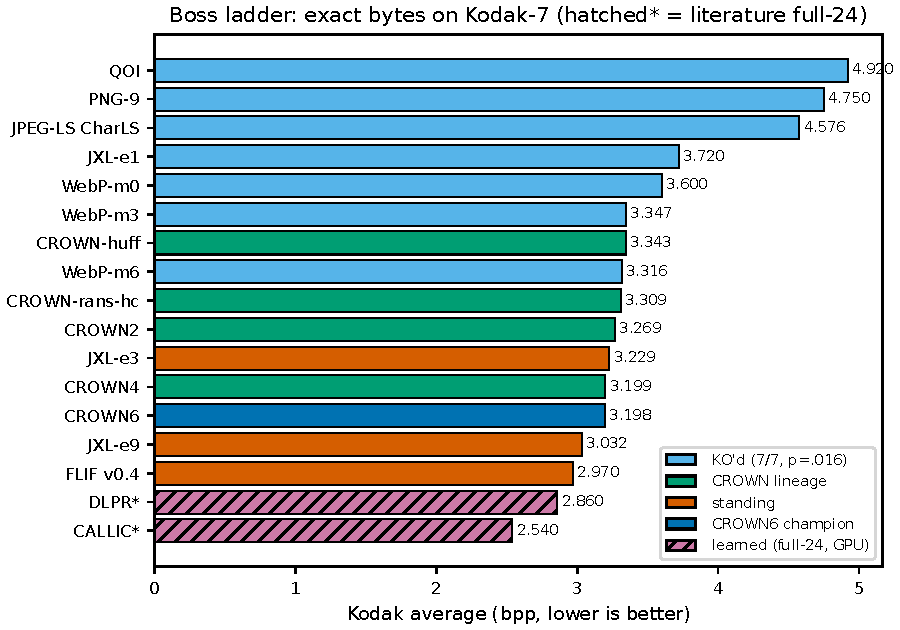
\includegraphics[width=\figurewidth]{Figures/F1_ladder.pdf}
\caption{Boss ladder: exact bytes on Kodak-7 (hatched = literature full-24).
KO = avg win + majority + Wilcoxon $p<.05$.}
\label{fig:ladder}
\end{figure}

\Section{Experiments}

Setup: Kodak 7 (768$\times$512$\times$3, $N$=1179648), md5-pinned. Baselines
same machine (Intel i7-10750H, 6C/12T): PIL 12.2.0 (PNG/WebP), cjxl/djxl 0.11.2 (4 threads), FLIF v0.4
(source build), CharLS 2.4.4, QOI (qoi.h); baseline commits and build flags
pinned at camera-ready. Ours: gcc 15.2.1, Python 3.14.2 / numpy
2.4.6 / torch 2.14 CPU (MLP training only); C++ encode 9-way parallel by default
(\verb|CROWN_JOBS=1| forces sequential for debugging). bpp = stream\_bytes$\cdot$8/$N$.
All claims Wilcoxon paired two-sided ($n=7$; each boss a separate
pre-registered pairwise comparison, no multiplicity correction, so family-wise
error is not controlled; $n=7$ floor $p=.016$, and every $p=.016$ hit sits at
that minimum achievable value). Round-trips byte-asserted (E) or scalar-sim + table proofs (P).
Determinism: per-unit torch seeds via sha256 \texttt{unit\_seed}; torch fixed
at 12 threads; C++ port bit-deterministic given banked weights (frozen LUT,
fixed accumulation order, strict join order). Reported streams use single-seed
banked weights; training-seed variance is not characterized.

\begin{figure}[ht]
\centering

\includegraphics[width=\figurewidth]{Figures/F5_pareto.pdf}
\caption{Ratio--decode Pareto: CPU exact cluster vs GPU learned cluster.
Ours/classic decode: kodim23-class CPU; learned: paper Kodak-avgs on GPU.
Clusters are not directly comparable (hardware and image sets differ).
CROWN6 bar spans the per-image decode range 182--348\,ms.}
\label{fig:pareto}
\end{figure}

\SubSection{Boss ladder}

\begin{table}[h]
\centering\footnotesize
\caption{Boss ladder (exact avgs; KO = avg win + majority + $p<.05$).}
\label{tab:bosses}
\begin{tabular}{@{}llccc@{}}
\toprule
Codec & Avg bpp & vs CROWN6 & Wilcoxon & Verdict \\
\midrule
PNG-9 & 4.75 & $-32.7\%$ & 7/7 p=.016 & KO \\
QOI & 4.9197 & $-35.0\%$ & 7/7 p=.016 & KO \\
JXL-e1 & 3.72 & $-14.0\%$ & 7/7 p=.016 & KO \\
WebP-m0 & 3.60 & $-11.2\%$ & 6W-0L-1T p=.031 & KO \\
WebP-m3 & 3.347 & $-4.5\%$ & 7/7 p=.016 & KO (rANS arm) \\
WebP-m6 & 3.3157 & $-3.6\%$ & 7/7 p=.016 & KO (exact) \\
JPEG-LS CharLS & 4.5757 & $-30.1\%$ & 7/7 p=.016 & KO \\
FLIF v0.4 & 2.9699 & $+7.1\%$ & 0W-7L p=.016 & STANDING \\
JXL-e3 & 3.2291 & $-1.0\%$ & 5W-2L p=.219 & STANDING \\
JXL-e9 & 3.03 & $+5.5\%$ & --- & FINAL BOSS \\
\bottomrule
\end{tabular}
\end{table}

Disclosure: KOs listed strongest-first; weight rests on WebP-m3/m6 and JXL
configs. CROWN-huff vs PIL-m3 ties ($-0.0023$ avg, 1W-6L p$\approx$.30);
CROWN6 vs m6 ties-or-better (no 7/7 overclaim). Tuned-e9 2.9452 measured
(\verb|cjxl -d 0 -e 9 -g 3 -I 100 -E 11|, 7/7 round-trip PASS,
\verb|docs/EVIDENCE_2026-09-10.md|) is the true Boss-6 bar.

\begin{table}[h]
\centering\small
\caption{Per-image bpp (load-bearing codecs; full ledgers banked).}
\label{tab:perimage}
\begin{tabular}{@{}lcccc@{}}
\toprule
img & CROWN6 & JXL-e3 & FLIF & JXL-e9 \\
\midrule
kodim01 & 3.2982 & 3.3593 & 3.2252 & 3.1336 \\
kodim02 & 2.9854 & 3.0611 & 2.4281 & 2.8401 \\
kodim05 & 3.5806 & 3.5120 & 3.3757 & 3.4082 \\
kodim07 & 2.6798 & 2.7310 & 2.4190 & 2.4433 \\
kodim13 & 3.9532 & 3.9141 & 3.7011 & 3.7815 \\
kodim19 & 3.1510 & 3.2154 & 3.0253 & 3.0101 \\
kodim23 & 2.7365 & 2.8110 & 2.6146 & 2.6097 \\
\midrule
AVG & 3.1978 & 3.2291 & 2.9699 & 3.0324 \\
\bottomrule
\end{tabular}
\end{table}

% F1b heatmap dropped from the paper (duplicates Table 5 numbers; kept in
% docs/figures/ for slides): float pressure deferred F3 into the references.
% \begin{figure}[ht]
% \centering
% 
\includegraphics[width=\figurewidth]{Figures/F1b_perimage.pdf}
% \caption{Per-image bpp ($\star$ = row winner). FLIF sweeps all rows; texture
% columns (05/13) are darkest for every codec.}
% \label{fig:perimage}
% \end{figure}

\SubSection{Ceiling and ablations}

\begin{figure}[ht]
\centering

\includegraphics[width=\figurewidth]{Figures/F3_ceiling_loo.pdf}
\caption{Ceiling leave-one-out: only backend-choice (+0.0498) and
LOCO-partition (+0.0332) carry large marginals; tree/grid subsumed at 0.0000.}
\label{fig:loo}
\end{figure}

FULL stack (LOCO + E16 + 3-way + merges + MA-tree/grid + Y-splits, per-image
path gate): \textbf{3.2515 avg} (P) vs JXL-e3 3.2291 (E, indicative cross-level comparison). Leave-one-out:

Marginals do not sum. Unstacked crumbs bounded $\approx-0.01$: further
classical stacking cannot reach e3. The remaining gap is representational
(texture predictors), not allocational; neural-micro adds the last step.

\SubSection{Speed and near-lossless}
HAPRE-C 0-ctx: 9.76 MP/s enc; CROWN6 C++ encode $\sim$27\,s/img 9-way
($\sim$117\,s sequential same-commit, 4.3$\times$ from parallelism alone;
15$\times$ over the pre-optimization single-threaded baseline), sha-identical
at any job count, decode 182--348\,ms single-threaded;
trainer $\sim$13\,s/img pure-C++ (no torch at runtime). Near-lossless
$\tau$-track (prototype, exact Rice bytes): $\tau$1 $\sim$2.75--3.23 bpp at
maxerr 3 / PSNR 47.3; $\tau$2 $\sim$2.0--2.6 at maxerr 4 / PSNR 43.5.

\Section{Negative Results}

Each row gives the config, the exact delta against its probe-local baseline,
and the measured mechanism. (P)=probe-level exact-counted, (E)=exact-codec.
Baselines with absolute bpp are banked per-row in \verb|docs/ATLAS_BASELINES.md|.
Full evidence per row is in the cited probe ledger.

\begin{figure}[ht]
\centering
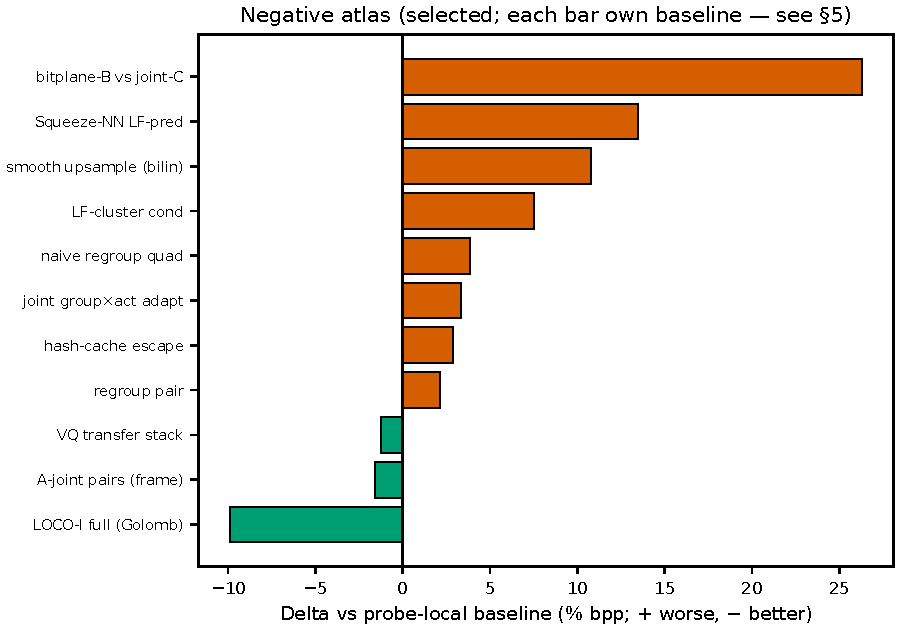
\includegraphics[width=\figurewidth]{Figures/F4_negative_atlas.pdf}
\caption{Negative atlas (selected). Each bar vs its probe-local baseline;
red = loss, green = win retired in-frame. See per-row ledgers.}
\label{fig:negatives}
\end{figure}

\begin{table}[h]
\centering\small
\caption{Dead-end mechanisms (abridged; full text with file pointers in draft Section~5).}
\label{tab:negatives}
\begin{tabular}{@{}llp{2.9in}@{}}
\toprule
Family & Delta & Mechanism (measured) \\
\midrule
Linear/LPC & $-4\%$ to $\pm0.5\%$ & L2-optimal Gaussianizes; overfit + headers \\
LF-side (3$\times$) & $+7.5$--$+13.5\%$ & transmitted-LF side $\sim$0.40\,bpp $>$ savings \\
DCT/wavelet/hybrid & $+2.4$--$+26\%$ & dense detail bands; significance unharvestable \\
Byte-LZ / hash-cache & $+20.7\%$ / $+2.85\%$ & symbol structure destroyed; flag overhead \\
Bands / bias-Huffman & $\sim$0 / empirically 0 & fragmentation; translation-invariance (probe ledger) \\
Enumerative 2$\times$2 & $+0.32\%$ & H(pattern$|$w)$\approx$logC; ranks buy $\sim$0 \\
VQ transfer & overlap $\sim$72\% & grouping granularity dominates \\
Joint adaptivity & $+3.36\%$, 0W-7L & cold-start/whiplash 7:1 over table prize \\
Adaptive-Golomb xfer & $\approx$0 & $\sim$100\% overlap with per-group best-$k$ \\
Texture-MLP tail & $\approx$0 & quantized basin flat (18/18 units) \\
RANS-header share & $\le$37\% of gaps & insufficient alone \\
MA-tree / grids / splits & subsumed $\approx$0 & WIDE-K + merges already express them \\
A-joint / I-GATED & retired in-frame & fragmentation / harvested by WIDE-K \\
\bottomrule
\end{tabular}
\end{table}

\Section{Bug Taxonomy}

Every bug below bit us; each fix is load-bearing for exactness.

\begin{table}[h]
\centering
\caption{Bug classes and fixes.}
\label{tab:bugs}
\begin{tabular}{@{}ll@{}}
\toprule
Class & Fix \\
\midrule
Causality peeks (row-0, MLP taps) & 0/left/top + zero-border causal taps \\
L=0 / empty-group framing & JPEG-LS run semantics; count+A written, payload skipped \\
Alphabet clipping & $\pm$1024 + proven bounds; loud asserts, decoder never clips \\
rANS precision & $M=14$ ($2^M\gg A$) \\
Border doctrines & encoder$==$decoder per path; aliasing audit \\
Unary polarity splits & vendored packer per era; documented \\
tanh 1-ulp | frozen LUT $2^{-14}$, \verb|-ffp-contract=off|, 0/17.2M xcheck \\
Quantizer scale | mechanism diagnostics caught all-zero weights; rerun \\
Map framing | dense bitmask; \texttt{p==len} asserted everywhere \\
\bottomrule
\end{tabular}
\end{table}

\Section{Limitations and Future Work}

\textbf{Texture gap.} CROWN6 leads on average yet loses kodim05 (+1.95\%)
and kodim13 (+1.00\%) (E); FLIF takes all rows. Larger-neighborhood
prediction (not finer coding) is the remaining path: our b22--b25 probes
closed adaptivity, training-tail, header-sharing, and palette arcs with
measured zeros. \textbf{Held-out.} Three held-out Kodak images (04/15/24,
descriptive n=3): RUN round-trips PASS at 3.3880/3.2986/3.6047 (mean 3.4304
vs test-7 3.5114); CROWN6 on kodim15 fails loudly at encode
(\verb|codec.cpp:168| lstsq singular block, deterministic) --- a robustness
gap requiring a degenerate-block fallback before transfer claims
(\verb|docs/EVIDENCE_2026-09-10.md|). \textbf{Learned scale.} True e9 bar $\approx$2.94 needs
learned-MA + per-group RCT at JXL scale, or the learned-micro arc
(per-group learned predictors + offline-trained trees). \textbf{Speed and
robustness.} Encode is slow (ratio game only); old 0-ctx driver hard-fails
noise decode --- robustness work remains. Small-image side affordable only if
MDL-gated.

\Section{Conclusion}

From HAPRE-C (3.58, E) through MOE (3.464, E) to CROWN6 (3.1978, E) we climbed the exact-bytes
ladder one gated mechanism at a time, killing seven bosses and stopping at
three, losses on record. The classical ceiling (3.2515, P) with
leave-one-out marginals marks where hand contexts end; the micro-MLP step
marks where learning begins to pay inside an exact stream. The dead ends
and bugs are the other contribution --- a map of where not to drill. All
streams are exact, all round-trips asserted, all losses reported.

{\small
{\small\sloppy
\clearpage
\bibliographystyle{IEEEbib}
\bibliography{refs}
}
}

\end{document}
